\section{Benchmark NIST-11 "Intersecting Interfaces"}
\label{sec:bench-11}

The solution to this elliptic problem contains a severe
singularity that poses a challenge to adaptive methods.
The equation solved is given by (Note: we need more description...)

\begin{equation} \label{intersecting}
-\nabla \cdot (a(x,y) \nabla u) = 0 
\end{equation}
where the parameter $a$ is piecewise-constant,
$a(x,y) = R$ in the first and third quadrants,
and $a(x,y) = 1$ in the remaining two quadrants.
The domain of this problem is $\Omega = (-1, 1)^2$, equipped with
Dirichlet boundary conditions given by the exact solution.

The exact solution:
\begin{equation}\label{exact-nist-11}
u(x,y) = r^{a} \mu
\end{equation}

The solution of NIST-11 is shown in Fig. \ref{fig:sln-nist11}.

\begin{figure}[!ht]
\centering
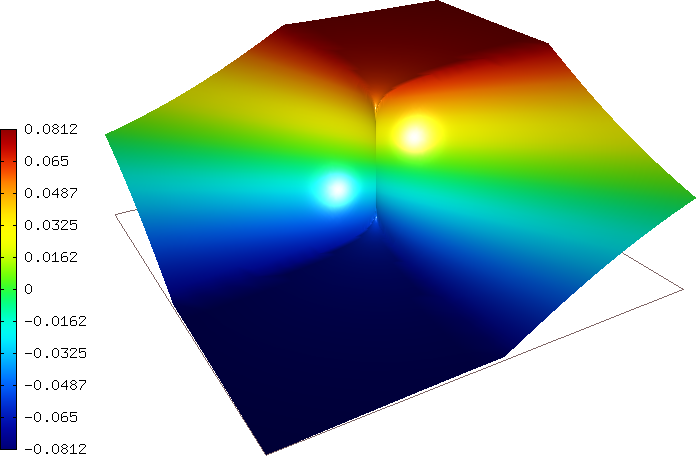
\includegraphics[height=6cm]{nist/nist-11/solution.png}
\caption{The solution to NIST-11 benchmark problem.}
\label{fig:sln-nist11}
\end{figure}

The goal of the benchmark is to reach a relative error below
$0.5$~\% in the $H^1$-norm with as few DOFs as possible.
We begin with adaptive $hp$-FEM with possible anisotropic refinements.
The initial mesh is shown in Fig. \ref{fig:nist-11-hp-aniso} (left).
In a few adaptivity steps, the polynomial degree of elements is increased
anisotropically.
The resulting mesh with 591 DOF is shown in Fig. \ref{fig:nist-11-hp-aniso} (right).

\begin{figure}[!ht]
\centering
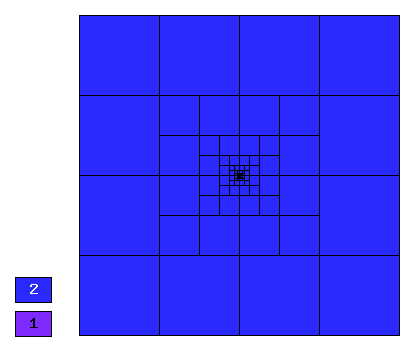
\includegraphics[height=5cm]{nist/nist-11/mesh_hp_aniso_init.png}\ \
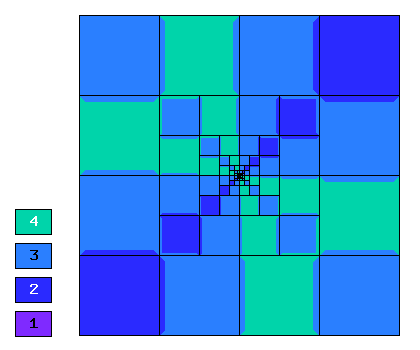
\includegraphics[height=5cm]{nist/nist-11/mesh_hp_aniso.png}
\vspace{-2mm}
\caption{Initial mesh (left) and final mesh (right) for $hp$-FEM with anisotropic refinements.}
\label{fig:nist-11-hp-aniso}
\end{figure}

The final relative error estimate in $H^1$-norm was 4.7087e-01 \%,
and it was identical to the exact error in all printed digits.
We also solved this benchmark with adaptive $h$-FEM
with linear (left) and quadratic (right)
elements, with anisotropic refinements enabled.
Final meshes for the $h$-FEM computations are shown
in Fig. \ref{fig:nist-11-h-aniso}.

\begin{figure}[!ht]
\centering
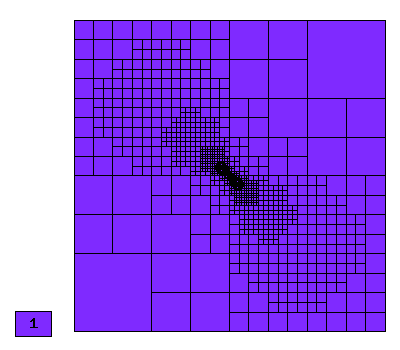
\includegraphics[height=5cm]{nist/nist-11/mesh_h1_aniso.png}\ \
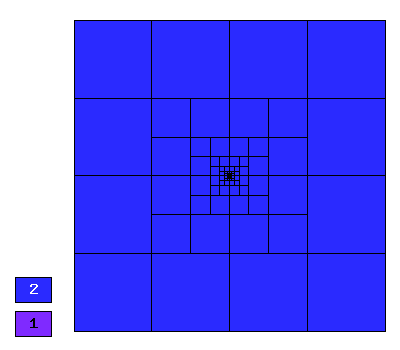
\includegraphics[height=5cm]{nist/nist-11/mesh_h2_aniso.png}
\vspace{-2mm}
\caption{Final mesh for $h$-FEM anisotropic refinements with linear and quadratic elements.}
\label{fig:nist-11-h-aniso}
\end{figure}

Figs. \ref{fig:nist-11-conv} compare all
three approaches to automatic adaptivity from the point
of view of DOF and CPU convergence.

\begin{figure}[!ht]
\centering
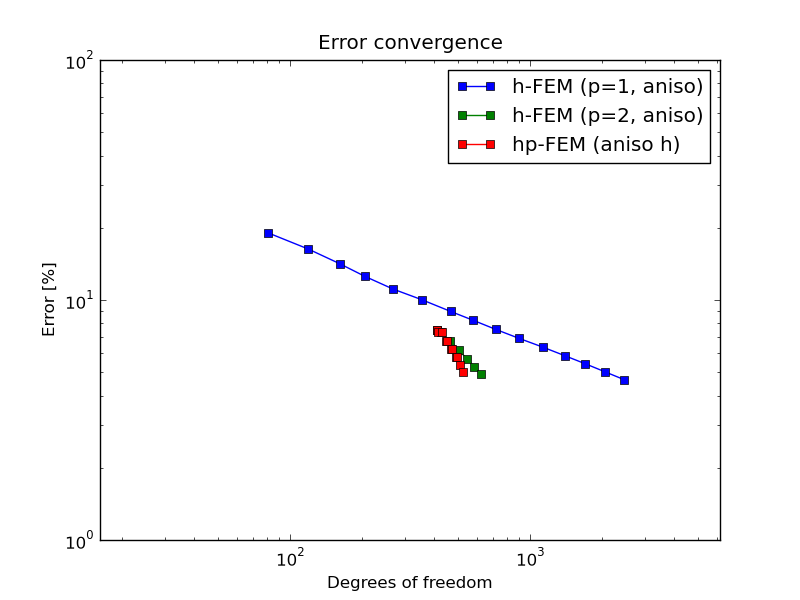
\includegraphics[height=5cm]{nist/nist-11/conv_dof_aniso.png}\ \
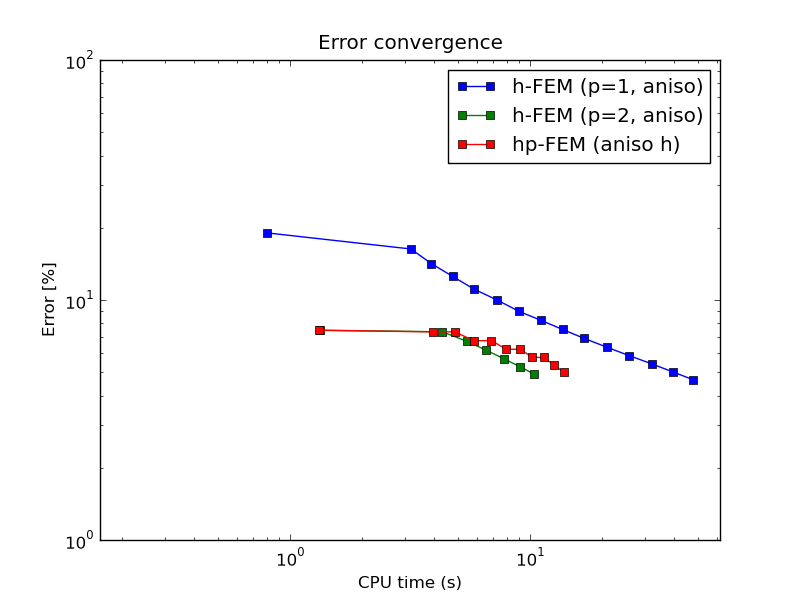
\includegraphics[height=5cm]{nist/nist-11/conv_cpu_aniso.png}
\caption{DOF and CPU time convergence graphs.}
\label{fig:nist-11-conv}
\end{figure}

